\section{Economic performance}\label{sec:econ}
\begin{table}[H]
\centering
\caption{Performance at hour 0 (S1, S3) and over 200 years (E4, quota scan).}\label{tab:econ}
\small
\begin{tabular}{@{}p{0.3\linewidth}p{0.62\linewidth}@{}}
\toprule
Measure & Result \\
\midrule
Access & Every settlement has an open route at every hour of 200 years; 24-hour availability $1.000$ at hours 0 and 300. Outer clients trade continuously on their operator's local market, whose quotes stayed inside the band in both price runs \\
Completion: transfer to hub & Credit $0.56\h$ (Ceres), $0.85\h$ (Jupiter, median), $4.17\h$ (Neptune); final after $1.11$, $1.70$, $8.35\h$ \\
Completion: order to fill & Inner: cutoff wait $\le1.5\h$, clearing lag $\le0.89\h$. Outer: cutoff wait $\le6\h$, clearing lag $\le4.35\h$ \\
Completion: price runs & Rising $15.2\h$, falling $26.0\h$ from first move until every top-up is final \\
Communication & 398 originations a day on average, 468 on the worst day of 200 years, of 600; worst link load $5.6\%$ of capacity \\
Capital & Initial margin $1.33$--$3.01\%$ of notional; prefunded resources $57.40$ for $1{,}500$ gross notional ($3.8\%$, breakdown in E3), against $4.6\%$ for a single three-hour batch \\
Recovery & S2: service restored within the incident plus one round trip; no obligation lost; collateral never negative \\
\bottomrule
\end{tabular}
\end{table}

\begin{figure}[H]
\centering
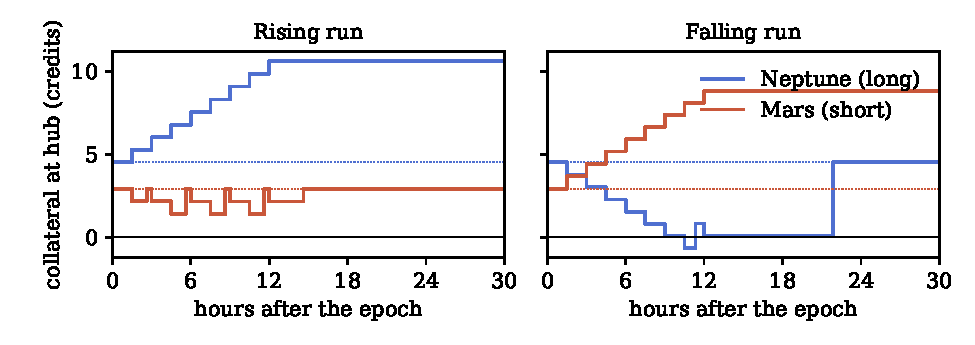
\includegraphics[width=\linewidth]{fig_runs.pdf}
\vspace{-14pt}
\caption{S1 price runs, weighted equally: collateral at the hub (solid) against initial margin (dotted). The losing side receives calls and tops up; Neptune's top-ups take a round trip of about 8 hours, yet its collateral never goes negative.}
\end{figure}
\vspace{-6pt}
\section{Continuing operation}\label{sec:cont}
MPX runs indefinitely on the frozen elements. Every closure in the next 200 years is known, so R1 schedules re-pins in advance: about $7.9$ a year for Mercury, $2.8$ for Venus, $1.6$ for Earth and fewer than one for the rest, at one origination each. Copy counts are recomputed for every send from the predicted geometry. The quota is budgeted on a rolling 24-hour window, with 132 originations held in reserve on the worst day. The fund is recalibrated with each book change, members recertify liquidity monthly, and timestamps are TDB throughout. The scenarios rerun at $+1$, $+10$ and $+100$ years and at the worst epoch of the 200-year scan with balances reset; completion times stay within $4.0\h$ of hour 0 and funding is conserved in every run (E5).

\section{Deployment assessment}\label{sec:deploy}
\textbf{What exists.} Every rule in this paper runs on the brief's frozen model: propagation, the 200-year closure scan, routing, loss and delivery, the protocol engine with its ledgers, and the stress runs. Two independent implementations agree to the last reported digit, and the toolkit's eight checks pass.

\textbf{What deployment needs.} A clearing service at Earth (matching, the clearing ledger, the fund); a home ledger at each settlement; operators at Uranus and Neptune with their escrow prefunded at the hub; relay software that sends one aggregate receipt per hop per batch; signing keys registered for every settlement; atomic clocks keeping TDB; and the Mars standby with leases (R8f).

\textbf{Order of rollout.} (1) Earth hub and the fast tier, Mercury to Jupiter, with transfers and spot. (2) Saturn and the full batch. (3) Operators at Uranus and Neptune, with their local markets and escrow. (4) Futures and cross-planet swaps. (5) The Mars standby. (6) The delivery guarantee, once observed loss confirms the model's abandonment rates. Each step adds load the quota analysis already covers.

\textbf{Acceptance tests.} Each deadline message on time with probability at least $99.5\%$; at most 468 originations on any day; daily reconciliation showing zero difference in total funding across all ledgers; margin exceeded in at most $1\%$ of margin periods, checked monthly.

\textbf{Known gaps.} The brief refers to a reference propagator that the v1.3 archive does not contain; ours reproduces the epoch table to $4.7\times10^{-7}\AU$ and we report the gap to the organizers. Fixed ellipses drift from the real ephemeris by up to about $16$\,ms of light-time (\cref{sec:effects}). Probabilities assume independent launches, which incidents break; the rulebook covers incidents. The $30\%$ liquidity rule and the 6-hour outer cadence are deliberate costs, quantified in E5 and R2.

\section{Real-world effects omitted by the model}\label{sec:effects}
\textbf{1. Perturbations and the Earth--Moon wobble.} The brief propagates fixed ellipses. The JPL Horizons files in the data pack \cite{horizons} give each body's osculating elements one day after the epoch. Propagating the fixed epoch elements one day and comparing with the next day's elements shows divergences of $115\km$ for Earth, $86\km$ for Jupiter and $41\km$ for Neptune. Earth's deviation is dominated by the Moon: Earth orbits the Earth--Moon barycentre at $384{,}400/82.3 = 4{,}671\km$ \cite{folkner2009}, a $15.6$\,ms light-time effect that breaks the brief's 1\,ms tolerance within days. \emph{Assumption:} errors grow from these one-day values toward the lunar amplitude. \emph{Effect on MPX:} the 60\,s send-early margin is about 3{,}800 times larger, and predicted closure times shift by seconds to minutes against re-pins planned days ahead.

\textbf{2. Shapiro delay.} General relativity delays light passing the Sun by $(2GM/c^3)\ln\frac{r_1+r_2+d}{r_1+r_2-d}$ \cite{shapiro1964}, with $2GM/c^3=9.85\,\mu$s. Our worst hop, from Mercury at perihelion to a relay grazing the $0.10\AU$ exclusion, gains $57\,\mu$s; Neptune's whole route to Earth gains $38\,\mu$s. Both are well inside the 1\,ms tolerance, so the model's omission is safe for MPX.

\section{Related systems}\label{sec:related}
Each mechanism has a proven ancestor. Hop receipts and retries are the custody transfer of delay-tolerant networking, selected for NASA's LunaNet \cite{cerf,rfc9171}. Light-Cone Clearing generalizes frequent batch auctions \cite{budish2015}, with physics in place of IEX's $350\,\mu$s speed bump. Light-time settlement risk is Herstatt risk, and payment-versus-payment is the CLS remedy \cite{bisfx}. Tombstoned refunds and R8b are the receiver-signed refund and atomic swap of hash time-locked contracts \cite{htlc}. An Earth--Mars Bitcoin design also settles locally with light-time timelocks \cite{puente}; a sovereign-Mars proposal bans interplanetary currency transactions \cite{haqq}, which MPX shows to be unnecessary.

\section{Future work}\label{sec:future}
Not part of the rules: an equilibrium model of tier choice, price filtering from stale quotes, and location proofs beyond signed keys.

\begin{thebibliography}{9}\small
\bibitem{budish2015} E. Budish, P. Cramton, J. Shim. The high-frequency trading arms race. \emph{Quarterly Journal of Economics} 130(4), 2015.
\bibitem{pfmi} CPSS--IOSCO. \emph{Principles for Financial Market Infrastructures}, 2012 (Cover 2).
\bibitem{folkner2009} W. Folkner, J. Williams, D. Boggs. The planetary and lunar ephemeris DE 421. \emph{IPN Progress Report} 42-178, 2009.
\bibitem{gilbert2002} S. Gilbert, N. Lynch. Brewer's conjecture and consistent, available, partition-tolerant web services. \emph{SIGACT News} 33(2), 2002.
\bibitem{shapiro1964} I. Shapiro. Fourth test of general relativity. \emph{Physical Review Letters} 13, 1964.
\bibitem{brief} Gator Quant Hacks 2026, Quantitative Puzzles. \emph{MultiPlanetary Exchange System} participant brief and v1.3 data pack.
\bibitem{cerf} V. Cerf. An interplanetary internet. Lecture, Heidelberg Laureate Forum.
\bibitem{rfc9171} S. Burleigh, K. Fall, E. Birrane. Bundle Protocol Version 7. RFC 9171, IETF, 2022.
\bibitem{bisfx} BIS. FX settlement risk remains significant. \emph{BIS Quarterly Review}, December 2019.
\bibitem{htlc} Hashed time-lock contracts and atomic swaps; e.g. Garden Finance HTLC documentation.
\bibitem{puente} J. E. Puente, C. Puente. Bitcoin as an interplanetary monetary standard with proof-of-transit timestamping. arXiv:2508.20591, 2025.
\bibitem{haqq} J. Haqq-Misra. A model for economic freedom on Mars. arXiv:2406.10380, 2024.
\bibitem{horizons} NASA JPL Horizons, osculating elements, 2026-09-22 and 2026-09-23 TDB (data pack).
\end{thebibliography}
